%----------------------------------------
\begin{frame}[fragile]
  \frametitle{A rover: timelines} \small

\begin{lstlisting}[basicstyle=\ttfamily\tiny]
tasknet Rover2 {
  end = 400;

  timelines {
    arm         : atomic = 0;
    location    : state(home, target) = home;
    data        : cumulative [0.0, 50.0]  bounds [0.0, 100.0] = 0.0;
    battery     : rate       [10.0, 100.0] bounds [0.0, 100.0] = 60.0;
    temperature : rate       [5.0, 40.0]  bounds [0.0, 100.0] = 10.0;
  }
  ...
}
\end{lstlisting}

\vspace{0.2cm}
\begin{itemize}
\item {\bf atomic}: a $[0,1]$ claim, for mutual exclusion.
\item {\bf state}: an enumeration.
\item {\bf cumulative}: a number, changed in steps.
\item {\bf rate}: a number with a rate of change: a battery, a temperature.
\item The first interval must hold at all times. The {\bf bounds} clamp.
\end{itemize}

\end{frame}

%----------------------------------------
\begin{frame}[fragile]
  \frametitle{A rover: tasks} \small

\begin{columns}[T]
\begin{column}{0.49\textwidth}
\begin{lstlisting}[basicstyle=\ttfamily\tiny]
taskdef drive_def {
  pre {
    battery in [60.0, 100.0];
    temperature in [10.0, 40.0];
  }
  impacts {
    maint { battery -~ 1.5; }
    post  { location = target; }
  }
}

task drive : drive_def {
  start_range    [100, 120];
  end_range      [130, 160];
  duration_range [30, 40];
}
\end{lstlisting}
\end{column}
\begin{column}{0.49\textwidth}
\begin{lstlisting}[basicstyle=\ttfamily\tiny]
task collect {
  duration_range [20, 30];
  pre {
    location = target;
    battery in [60.0, 100.0];
    arm = 0;
  }
  impacts {
    maint { arm += 1;
            battery -~ 0.5; }
    post  { data += 40.0; }
  }
}

optional task charge : charge_def {
  duration_range [60, 70];
}
\end{lstlisting}
\end{column}
\end{columns}

\vspace{0.1cm}
{\tt -\~{}} / {\tt +\~{}} change a {\bf rate}; {\tt +=} and {\tt =} change a {\bf value}.
An {\bf optional} task is scheduled only if it is needed.

\end{frame}

%----------------------------------------
\begin{frame}
  \frametitle{When impacts happen} \small

\begin{columns}[c]
\begin{column}{0.42\textwidth}
\centering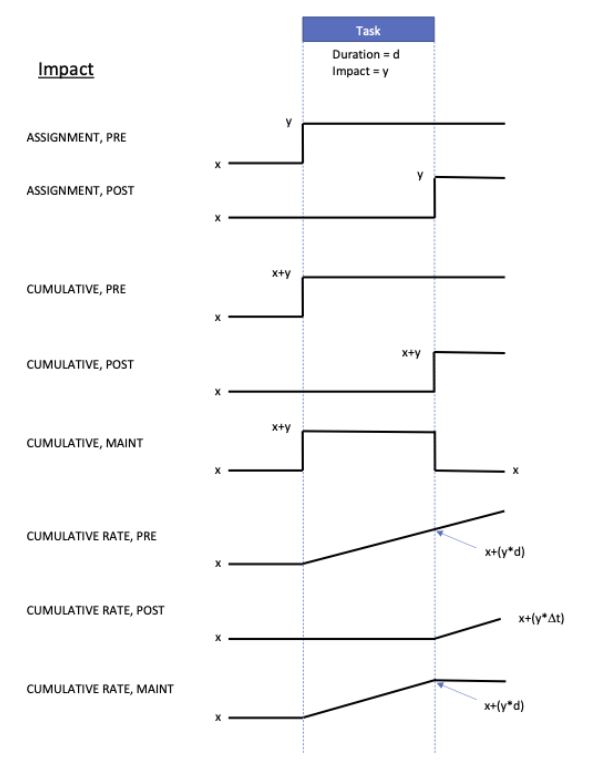
\includegraphics[height=0.78\textheight]{figures/impacts.png}
\end{column}
\begin{column}{0.56\textwidth}
\begin{itemize}
\item {\bf pre}: at the start, and stays.
\item {\bf post}: at the end, and stays.
\item {\bf maint}: at the start, undone at the end.
\end{itemize}

\vspace{0.3cm}
A task's own {\tt pre} sees the state {\em before} its impacts: {\tt collect} checks
{\tt arm = 0}, then runs with {\tt arm = 1}.

\vspace{0.3cm}
These are \mexec{}'s semantics, as best we understand them.
\end{column}
\end{columns}

\end{frame}

%----------------------------------------
\begin{frame}[fragile]
  \frametitle{Constraints and properties} \small

\begin{lstlisting}[basicstyle=\ttfamily\tiny]
constraints {
  prop not_charge_drive:   always not (active(charge) and active(drive));
  prop not_charge_collect: always not (active(charge) and active(collect));
  prop temperature10:      always temperature >= 10;
}
\end{lstlisting}

{\bf Constraints} restrict which schedules are valid.

\pause
\vspace{0.3cm}

\begin{lstlisting}[basicstyle=\ttfamily\tiny]
properties {
  prop target_reached: eventually (location = target and data >= 30);
  prop drive_charge:   always (active(drive) -> eventually active(charge));
  prop temperature:    always temperature >= 10;
}
\end{lstlisting}

{\bf Properties} are proved for {\em all} valid schedules, or refuted with a counterexample.

\vspace{0.2cm}
Past-time operators too: {\tt since}, {\tt once}, {\tt sofar}.

\end{frame}

%----------------------------------------
\begin{frame}
  \frametitle{The schedule} \small

\vspace{-0.15cm}
{\centering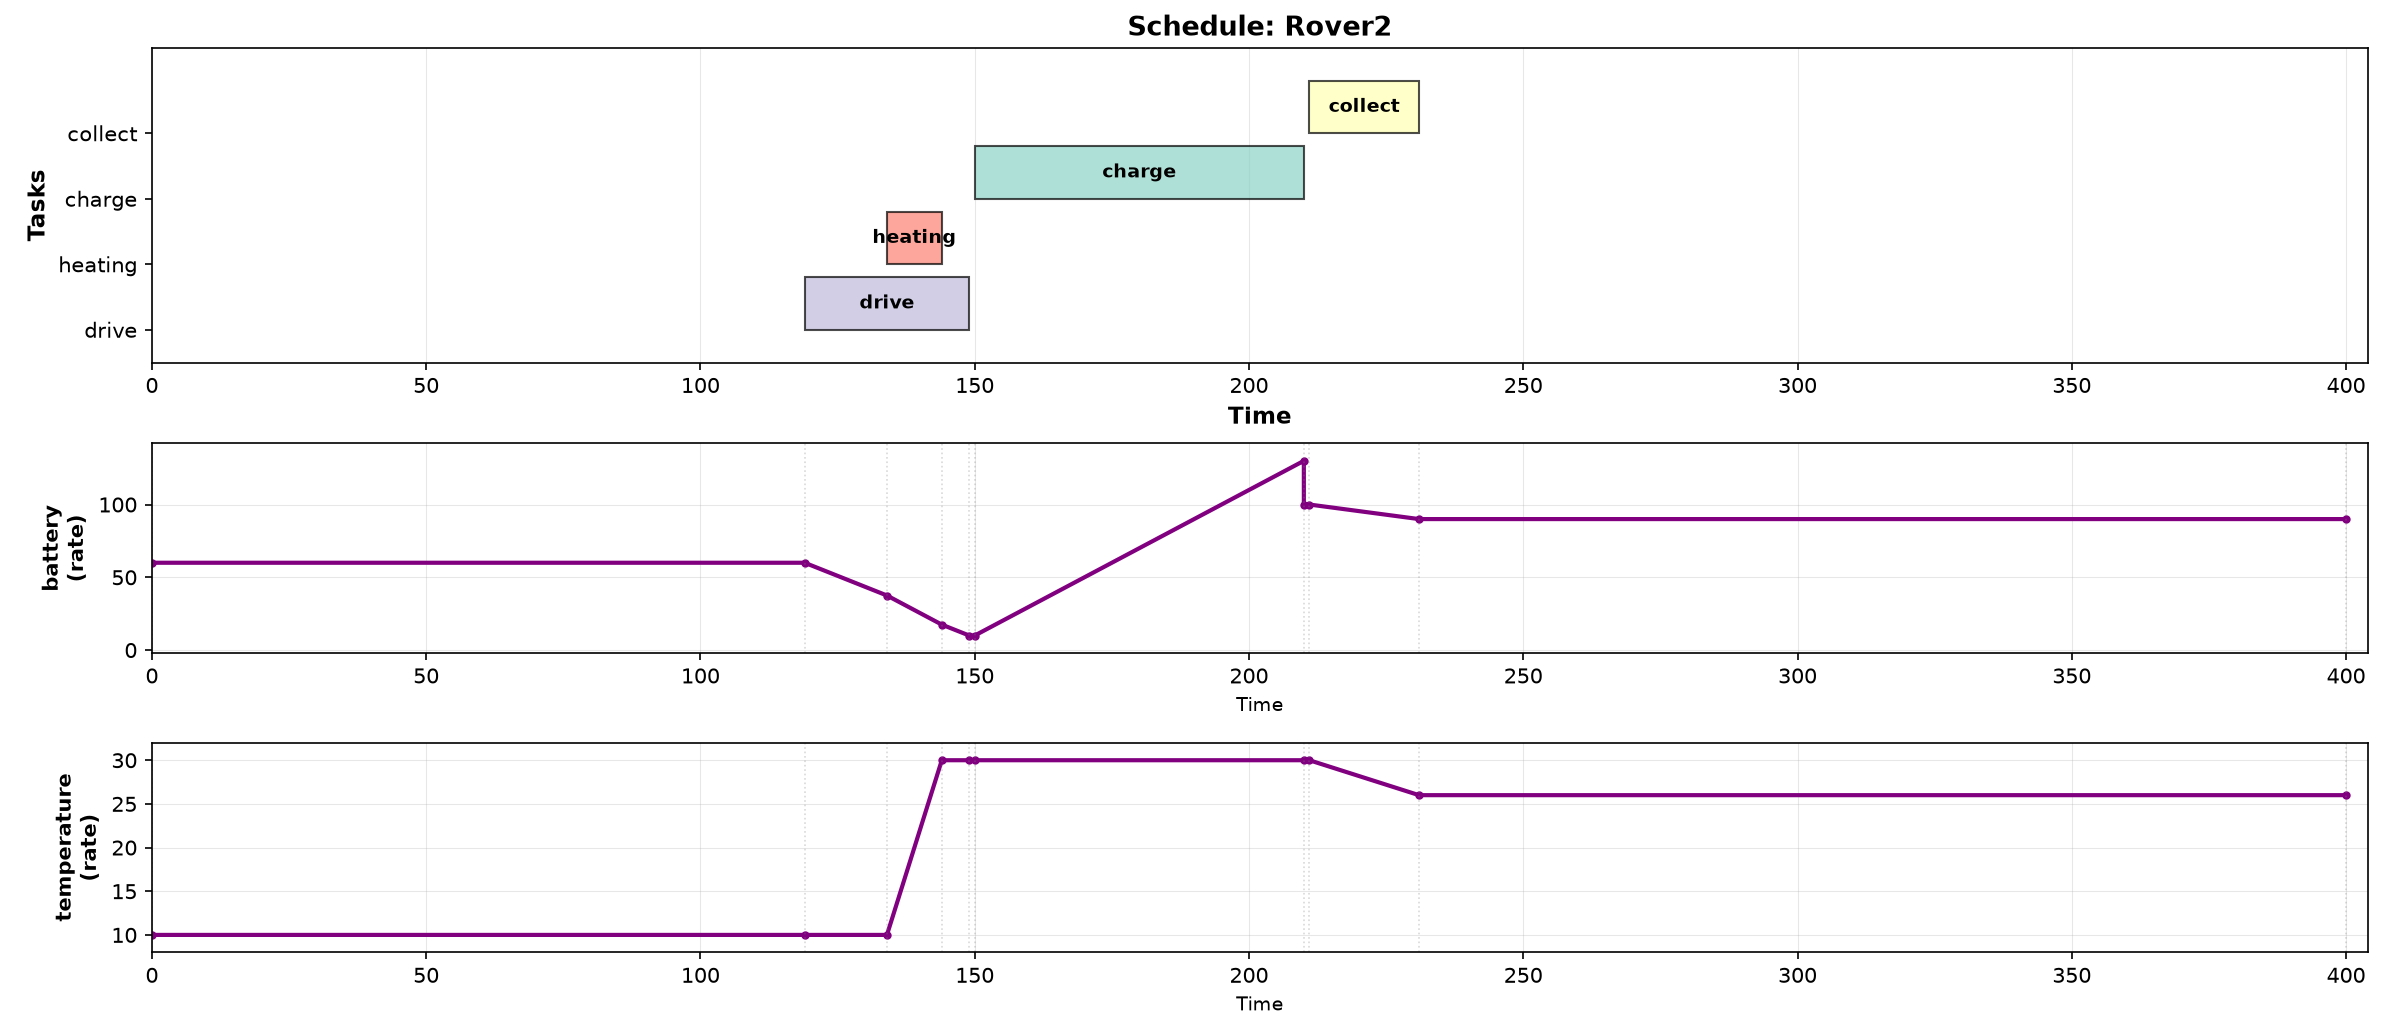
\includegraphics[width=\textwidth]{figures/rover2-timeline.png}\par}

\vspace{0.1cm}
Drive first, from the 60\% we start with, down to 10\%. Then charge to 100\% and collect.
{\tt heating} keeps the temperature up.
Charging first would waste most of it: the battery is full after 20 of its $\ge 60$ time units.

\end{frame}

%----------------------------------------
\begin{frame}
  \frametitle{The properties} \small

\vspace{-0.1cm}
{\centering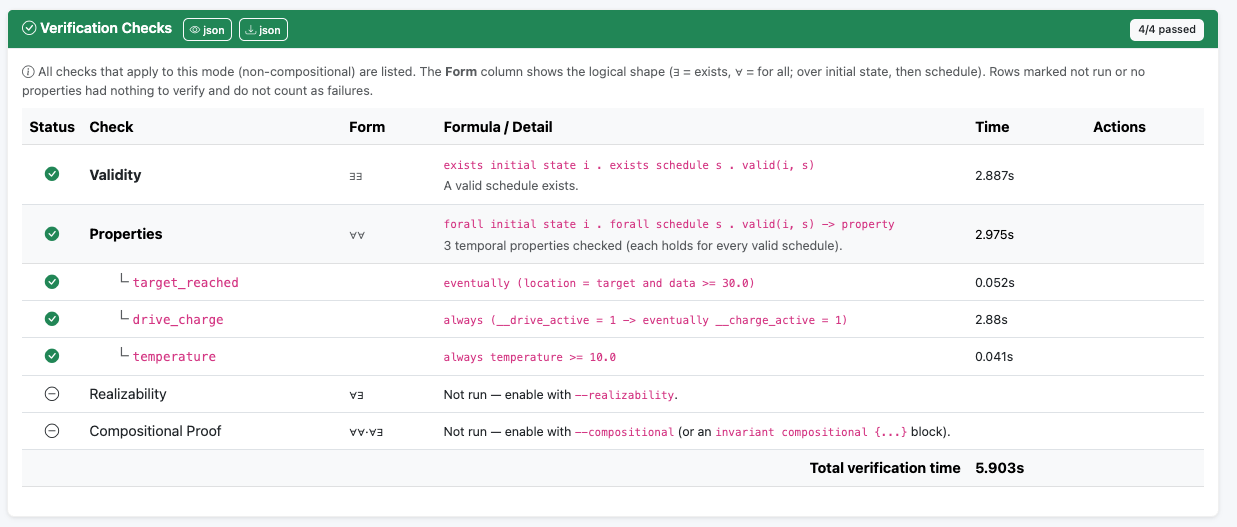
\includegraphics[width=\textwidth]{figures/rover2-results.png}\par}

\vspace{0.2cm}
Validity and the three properties, each with its logical form. 6 seconds in total.

\end{frame}

%----------------------------------------
\begin{frame}[fragile]
  \frametitle{When there is no schedule} \small

Ask for {\tt charge} to come first:

\begin{lstlisting}
task drive : drive_def {
  ...
  after charge;
}
\end{lstlisting}

\begin{lstlisting}[style=shell,basicstyle=\ttfamily\tiny]
=== Phase 1: Validity Check (EE) ===
UNSAT CORE (126 conflicting constraints)
  ...
  1. task_start_range: task 'drive' start must be in [100,120]
  2. task_end_range: task 'drive' end must be in [130,160]
  3. task_duration_range: task 'drive' duration must be in [30,40]
  4. dependency_after: 'drive' after 'charge'
  ...
  6. task_duration_range: task 'charge' duration must be in [60,70]
\end{lstlisting}

Charging first fills the battery (clamped at 100), {\tt drive} takes it to at most 55, and
{\tt collect} needs 60. There is only one {\tt charge}. Every constraint is labelled, so the
core reads back as the spec.

\end{frame}
